\documentclass[9pt,dvipsnames]{beamer}
\usepackage[T1]{fontenc}
\usepackage{libertinus}
\usepackage{amsmath}
\usepackage[most]{tcolorbox}

\usepackage{hyperref}

\usepackage{xcolor}  
\newcommand{\cb}[1]{{\color{CadetBlue}#1}}


\usetheme{Berkeley}
% \setbeamertemplate{footline}[frame number]
\setbeamertemplate{navigation symbols}{}


\title{CSE574 Introduction to Machine Learning}
\subtitle{Continual Learning}
\author{Jue Guo}
\institute{University at Buffalo}
\date{\today}

\begin{document}
\begin{frame}
    \titlepage
\end{frame}

\begin{frame}
    \frametitle{Outline}
    \tableofcontents
\end{frame}

\section{Abstract}
\begin{frame}{Abstract}
    To cope with real-world dynamics, an intelligent agent needs to incrementally acquire, update, accumulate, and exploit knowledge throughout its lifetime.
    \begin{itemize}
        \item \textbf{continual learning}, a fundation for AI systems to develop themselves adaptively. In a general sense, continual learning is explicitly limited by \textbf{catastrophic forgetting}, where learning a new task usually results in a dramatic performance degradation of the old tasks.
    \end{itemize}
\end{frame}

\section{Introduction}
\begin{frame}{Introduction}
    Learning is the basis for intelligent systems to accommodate environments. In response to external changes, evolution has empowered human and other organisms with strong adaptability to continually acquire, update, accumulate and exploit knowledge. Naturally we expect artifical intelligence (AI) systems to adapt in a similar way.
    \begin{itemize}
        \item This motivates the study of \textbf{continual learning}, where a typical setting is to learn a sequence of contents one by one and behave as if they were observed simultaneously. Such contents could be new skills, new examples of old skills, different environments, different contexts, etc., with particular realistic challenges incorporated.
        \item As the contents are provided incrementally over a lifetime, continual learnming is also referred to as \textbf{incremental learning} or \textbf{lifelong learning} in much of the literature, without a strict distinction.
    \end{itemize}
\end{frame}

\begin{frame}
    Unlike conventional machine learning models built on the premise of capturing a static data distribution, continual learning is characterized by learning from dynamic data distributions. A major challenge is known as \textbf{catastrophic forgetting}, where adaptation to a new distribution generally results in a largely reduced ability to capture old ones.
    \begin{itemize}
        \item This dilemma is a facet of the trade-off between \textbf{learning plasticity} and \textbf{memory stability}: an excess of the former interferes with the latter, and vice versa. A desirable solution for continual learning should obtain strong \textbf{generalizability} to accommodate distribution differences within and between tasks.
        \item A naive baseline, retraining all old training samples makes it easy to address the above challenges, but creates huge computational and storage overheads (as well as potential privacy issues).
    \end{itemize}
    In fact, continual learning is primarily intended to ensure the \textbf{resource efficiency} of model updates, perferably close to learning only new samples.
\end{frame}

\begin{frame}
    Numerous efforts have been devoted to addressing the above challenges, which can be conceptually seperated into five groups:
    \begin{enumerate}
        \item regularization-based approach
        \item replay-based approach
        \item optimization-based approach
        \item representation-based approach
        \item architecture-based approach
    \end{enumerate}
    These methods are \textit{closely connected}, e.g., regularization and replay ultimately act to rectify the gradient directions in optimization, and \textit{highly synergistic}, e.g., the efficacy of replay can be facilitated by distilling knowledge from the old model.
\end{frame}
\begin{frame}
    \begin{figure}[ht]
        \centering
        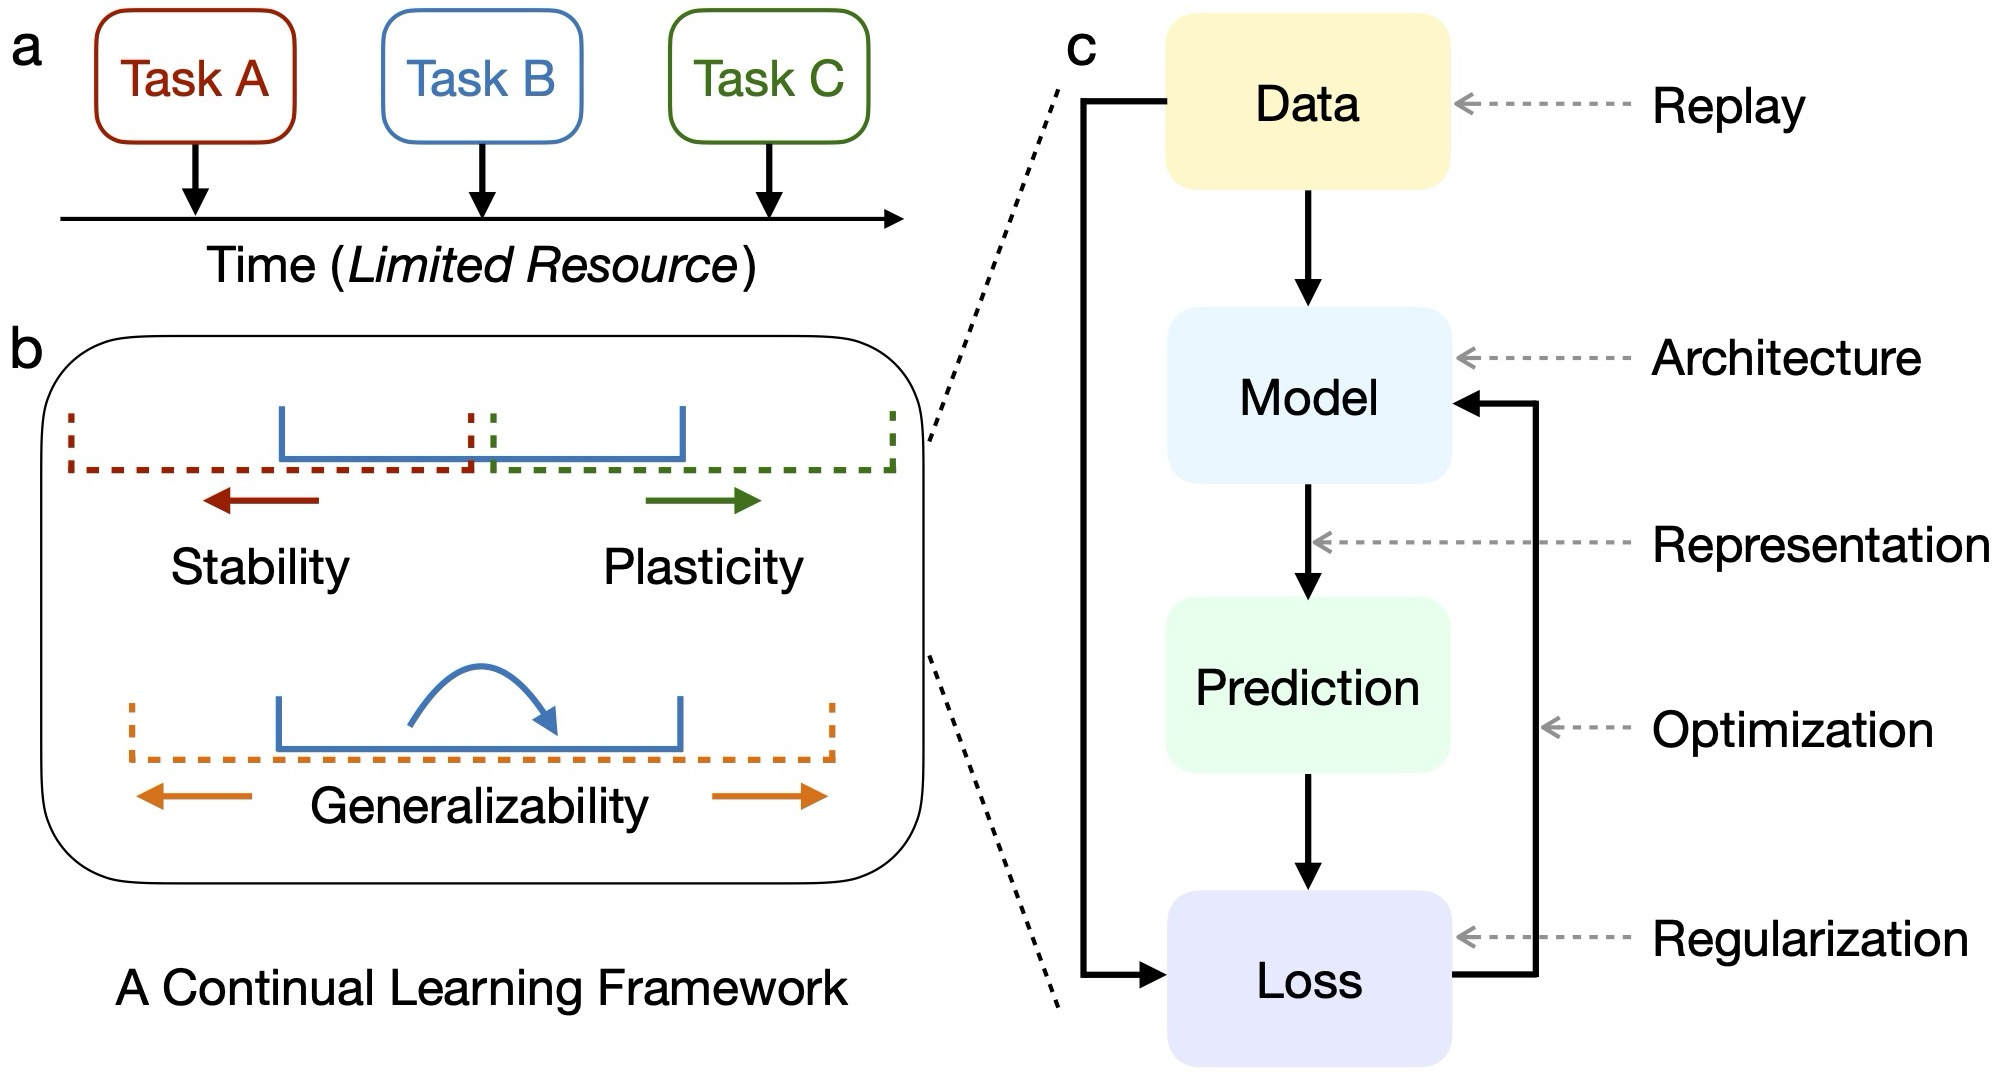
\includegraphics[width=0.5\linewidth]{imgs/cl_1.png}
        \caption{A conceptual framework of continual learning. \textbf{a}, Continual learning requires adapting to incremental tasks with dynamic data distributions. \textbf{b}, A desirable solution should ensure a proper balance between stability (red arrow) and plasticity (green arrow), as well as an adequate generalizability to intra-task (blue arrow) and inter-task (orange arrow) distribution differences. \textbf{c}, Representative strategies have targeted various aspects of machine learning.}
    \end{figure}
\end{frame}
\begin{frame}
    Realistic applications present particular challenges for continual learning, which can be categorized into \textit{scenario complexity} and \textit{task specificity}.
    \begin{itemize}
        \item \textcolor{red}{As for the former}, for example, the task oracle (i.e., which task to perform) is probably missing in training and testing, and the training samples might be introduced in tiny batches or even one pass. Due to the expense and scarcity of data labeling, continual learning needs to be effective for few-shot, semi-supervised and even unsupervised scenarios.
        \item \textcolor{red}{As for the latter}, although current advances mainly focus on visual classification, other vision domains such as object detection, semantic segmentation and image generation, as well as other related fields, such as reinforcement learning (RL), natural language processing (NLP) and ethic considerations, are receiving increasing attention with their own opportunities and challenges.
    \end{itemize}
\end{frame}

\section{Setup}
\begin{frame}{Setup}
    \begin{itemize}
        \item Basic formulation of continual learning
        \item Typica scenarios
        \item Evaluation metrics
    \end{itemize}
\end{frame}

\subsection{Basic Formulation}
\begin{frame}{Basic Formulation}
    Continual learning is characterized as learning from dynamic data distributions. In practice, training samples of different distributions arrive in sequence. A continual learning model parameterized by $\theta$ needs to learn corresponding task(s) with no or limited access to old training samples and perform well on their test sets.

    \begin{itemize}
        \item Formally, an incoming batch of training samples belonging to a task $t$ can be represented as $\mathcal{D}_{t, b}=\left\{\mathcal{X}_{t, b}, \mathcal{Y}_{t, b}\right\}$, where $\mathcal{X}_{t, b}$ is the input data, $\mathcal{Y}_{t, b}$ is the data label, $t \in \mathcal{T}=\{1, \cdots, k\}$ is the task identity and $b \in \mathcal{B}_{t}$ is the batch index $\left(\mathcal{T}\right.$ and $\mathcal{B}_{t}$ denote their space, respectively).
        \item Here we define a "task" by its training samples $\mathcal{D}_{t}$ following the distribution $\mathbb{D}_{t}:=p\left(\mathcal{X}_{t}, \mathcal{Y}_{t}\right)\left(\mathcal{D}_{t}\right.$ denotes the entire training set by omitting the batch index, likewise for $\mathcal{X}_{t}$ and $\mathcal{Y}_{t}$ ), and assume that there is no difference in distribution between training and testing. Under realistic constraints, the data label $\mathcal{Y}_{t}$ and the task identity $t$ might not be always available.
    \end{itemize}
    In continual learning, the training samples of each task can arrive incrementally in batches (i.e., $\left\{\left\{\mathcal{D}_{t, b}\right\}_{b \in \mathcal{B}_{t}}\right\}_{t \in \mathcal{T}}$ ) or simultaneously (i.e., $\left\{\mathcal{D}_{t}\right\}_{t \in \mathcal{T}}$ ).
\end{frame}

\subsection{Typical Scenario}
\begin{frame}{Typical Scenario}
    According to the division of incremental batches and the availability of task identities, we detail the typical continual learning scenarios as follows:
    \begin{itemize}
        \item \textit{Instance-Incremental Learning} (IIL): All training samples belong to the same task and arrive in batches.
        \item \textit{Domain-Incremental Learning} (DIL): Tasks have the same data label space but different input distributions. Task identities are not required.
        \item \textit{Task-Incremental Learning} (TIL): Tasks have disjoint data label spaces. Task identities are provided in both training and testing.
        \item \textit{Class-Incremental Learning} (CIL): Tasks have disjoint data label spaces. Task identities are only provided in training.
        \item \textit{Task-Free Continual Learning} (TFCL): Tasks have disjoint data label spaces. Task identities are not provided in either training or testing.
        \item \textit{Online Continual Learning} (OCL): Tasks have disjoint data label spaces. Training samples for each task arrive as a one-pass data stream.
        \item \textit{Blurred Boundary Continual Learning} (BBCL): Task boundaries are blurred, characterized by distinct but overlapping data label spaces.
        \item \textit{Continual Pre-training} (CPT): Pre-training data arrives in sequence. The goal is to improve the performance of learning downstream tasks.
    \end{itemize}
\end{frame}

\begin{frame}
    \begin{figure}[ht]
        \centering
        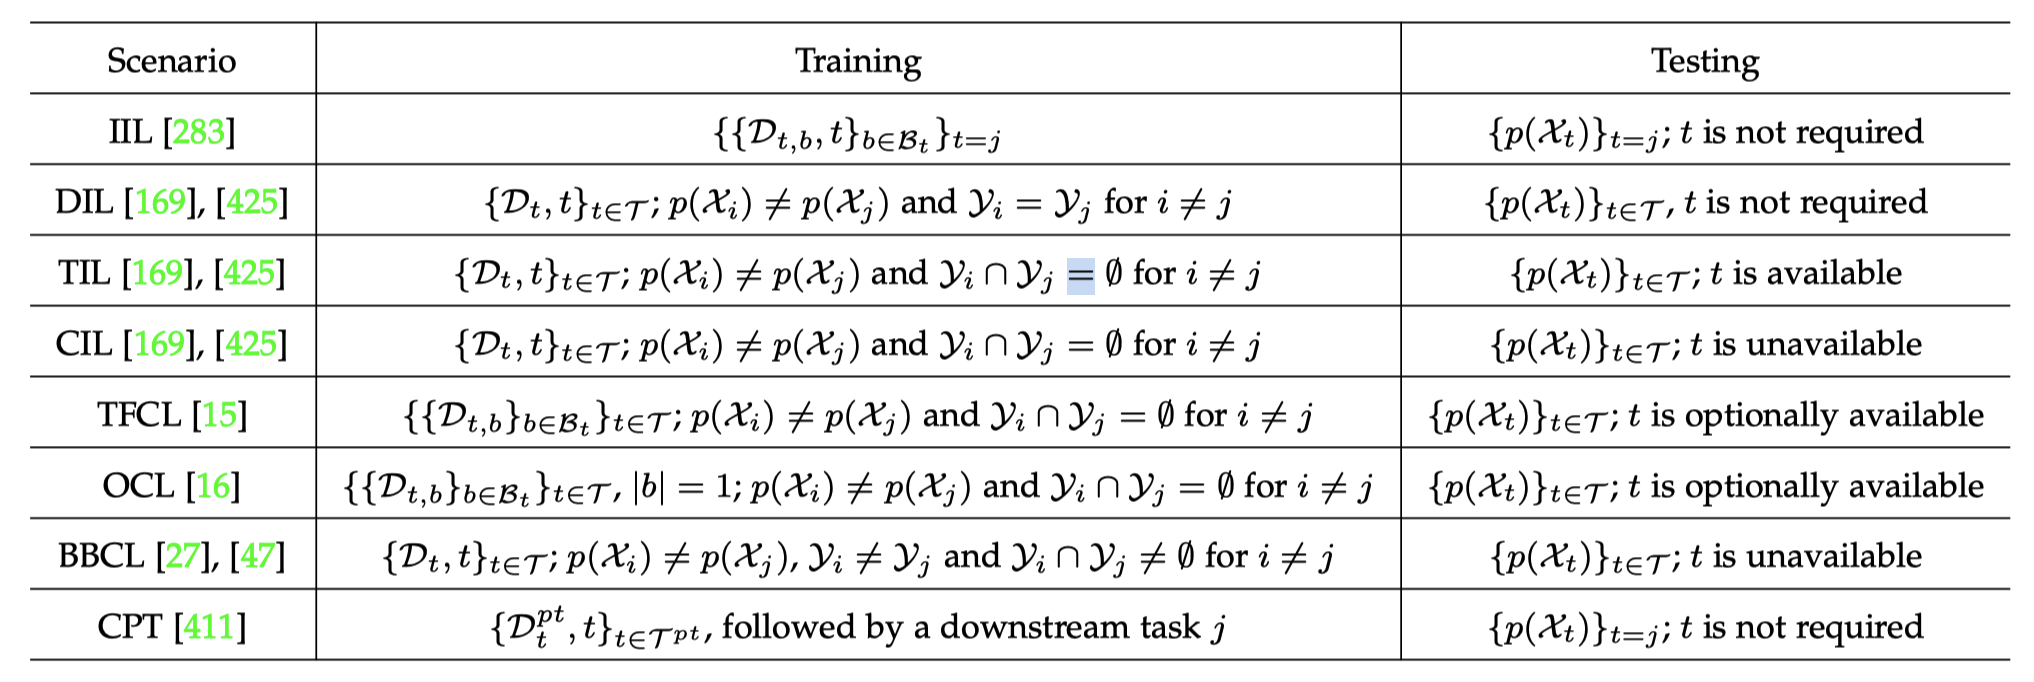
\includegraphics[width=\linewidth]{imgs/cl_2.png}
        \caption{A formal comparison of typical continual learning scenarios. $\mathcal{D}_{t, b}$ : the training samples of task $t$ and batch $b .|b|$ : the size of batch $b . \mathcal{B}_{t}$ : the space of incremental batches belonging to task $t \cdot \mathcal{D}_{t}$ : the training set of task $t$ (further specified as $\mathcal{D}_{t}^{p t}$ for pre-training). $\mathcal{T}$ : the space of all incremental tasks (further specified as $\mathcal{T}^{p t}$ for pre-training). $\mathcal{X}_{t}$ : the input data in $\mathcal{D}_{t} . p\left(\mathcal{X}_{t}\right)$ : the distribution of $\mathcal{X}_{t} . \mathcal{Y}_{t}$ : the data label of $\mathcal{X}_{t}$.}
    \end{figure}
\end{frame}
\begin{frame}
    If not specified, each task is generally assumed to have a sufficient number of labeled training samples, i.e., Supervised Continual Learning.
    \begin{itemize}
        \item According to the provided $\mathcal{X}_{t}$ and $\mathcal{Y}_{t}$ in each $\mathcal{D}_{t}$, continual learning can be further categorized into zero-shot, few-shot, semi-supervised, open-world (i.e., to identify unknown classes and then incorporate their labels)  and un-/self-supervised scenarios.
    \end{itemize}
    Besides, other practical challenges have been considered and incorporated,
    \begin{itemize}
        \item such as multiple labels , noisy labels, hierarchical granularity and sub-populations , mixture of task similarity , long-tailed distribution , domain alignment , domain shifting, anytime inference, novel class discovery, multi-modality, etc.
    \end{itemize}
    Some recent work has focused on various combinations of these scenarios, as a way of better simulating the complexity of the real world.
\end{frame}

\subsection{Evaluation Metric}
\begin{frame}{Evaluation Metric}
    In general, the performance of continual learning can be evaluated from three aspects: overall performance of the tasks learned so far, memory stability of old tasks, and learning plasticity of new tasks.
    \begin{itemize}
        \item Here we summarize the common evaluation metrics, using classification as an example. \textbf{Overall performance, Memory stability}, and \textbf{Learning plasticity}.
    \end{itemize}
\end{frame}

\begin{frame}
    \textbf{Overall performance} is typically evaluated by \textit{average accuracy} (AA) and \textit{average incremental accuracy} (AIA).
    \begin{itemize}
        \item Let $a_{k, j} \in[0,1]$ denote the classification accuracy evaluated on the test set of the $j$-th task after incremental learning of the $k$-th task $(j \leq k)$. The output space to compute $a_{k, j}$ consists of the classes in either $\mathcal{Y}_{j}$ or $\cup_{i=1}^{k} \mathcal{Y}_{i}$, corresponding to the use of multi-head evaluation (e.g., TIL) or single-head evaluation (e.g., CIL).
    \end{itemize}
    The two metrics at the $k$-th task are then defined as
    $$
        \mathrm{AA}_{k}=\frac{1}{k} \sum_{j=1}^{k} a_{k, j}
    $$
    $$
        \mathrm{AIA}_{k}=\frac{1}{k} \sum_{i=1}^{k} \mathrm{AA}_{i}
    $$
    where AA represents the overall performance at the current moment and AIA further reflects the historical variation.
\end{frame}

\begin{frame}
    \textbf{Memory stability} can be evaluated by \textit{forgetting measure} (FM) and \textit{backward transfer} (BWT). As for the former, the forgetting of a task is calculated by the difference between its maximum performance obtained in the past and its current performance:

    $$
        f_{j, k}=\max _{i \in\{1, \ldots, k-1\}}\left(a_{i, j}-a_{k, j}\right), \forall j<k .
    $$

    FM at the $k$-th task is the average forgetting of all old tasks:

    $$
        \mathrm{FM}_{k}=\frac{1}{k-1} \sum_{j=1}^{k-1} f_{j, k}
    $$

    As for the latter, BWT evaluates the average influence of learning the $k$-th task on all old tasks:

    $$
        \mathrm{BWT}_{k}=\frac{1}{k-1} \sum_{j=1}^{k-1}\left(a_{k, j}-a_{j, j}\right)
    $$

    where the forgetting is usually reflected as a negative BWT.
\end{frame}

\begin{frame}
    \textbf{Learning plasticity} can be evaluated by \textit{intransience measure} (IM) and \textit{forward transfer} (FWT). IM is defined as the inability of a model to learn new tasks, calculated by the difference of a task between its joint training performance and continual learning performance:

    $$
        \mathrm{IM}_{k}=a_{k}^{*}-a_{k, k}
    $$

    where $a_{k}^{*}$ is the classification accuracy of a randomlyinitialized reference model jointly trained with $\cup_{j=1}^{k} \mathcal{D}_{j}$ for the $k$-th task. In comparison, FWT evaluates the average influence of all old tasks on the current $k$-th task:

    $$
        \mathrm{FWT}_{k}=\frac{1}{k-1} \sum_{j=2}^{k}\left(a_{j, j}-\tilde{a}_{j}\right)
    $$

    where $\tilde{a}_{j}$ is the classification accuracy of a randomlyinitialized reference model trained with $\mathcal{D}_{j}$ for the $j$-th task. Note that, $a_{k, j}$ can be adapted to other forms depending on the task type, such as average precision (AP) for object detection, Intersection-over-Union (IoU) for semantic segmentation, Fréchet Inception Distance (FID) for image generation, normalized reward for reinforcement learning, etc, and the above evaluation metrics should be adjusted accordingly.
\end{frame}
\end{document}